\documentclass[conference]{IEEEtran}
\IEEEoverridecommandlockouts

\usepackage[T1]{fontenc}
\usepackage{cite}
\usepackage{amsmath,amssymb}
\usepackage{booktabs}
\usepackage{graphicx}
\usepackage{url}
\usepackage{xcolor}
\usepackage{multirow}
\usepackage{tikz}
\usetikzlibrary{positioning,arrows.meta,fit,calc,backgrounds}
\usepackage{pgfplots}
\pgfplotsset{compat=1.18}

% Numbers that depend on runs still in progress are marked and filled in last.
\newcommand{\pending}[1]{\textcolor{red}{#1}}

\definecolor{vis}{HTML}{DCE8F5}
\definecolor{llm}{HTML}{FBE8D3}
\definecolor{io}{HTML}{EFEFEF}
\definecolor{cue}{HTML}{E4F2E1}
\definecolor{s1}{HTML}{2A78D6}
\definecolor{s2}{HTML}{EB6834}
\definecolor{s3}{HTML}{1BAF7A}
\definecolor{s4}{HTML}{EDA100}
\tikzset{
  box/.style={draw, rounded corners=2pt, align=center, font=\footnotesize,
              inner sep=3pt, minimum height=7mm},
  arr/.style={-{Stealth[length=2mm]}, semithick},
}

\begin{document}

\title{Peekaboo-VL: Camera-Motion Text Hints and LoRA Letter Scoring\\for Drone Video Question Answering}

\author{\IEEEauthorblockN{Le Duc Minh}
\IEEEauthorblockA{\texttt{minh.leduc.0210@gmail.com}\\
MAVU Workshop @ WACV 2027 --- ReVA Drone Video Understanding Challenge}}

\maketitle

\begin{abstract}
Drone video is hard for video language models: the camera never stops
moving, objects are a few pixels wide, and many questions ask \emph{when}
something happens. The organizers' model, ReMoSense, adds learned
camera-motion tokens and reports a 3.9-point gain. We take the opposite
route: instead of teaching the model motion, we \emph{tell} it. A CPU probe
estimates the frame-to-frame camera motion in milliseconds and renders it
as one sentence in the benchmark's own answer vocabulary (``moving
forward'', ``panning left''). Fine-tuning Qwen3.5-9B with LoRA at 32
frames and reading the answer from the letter scores A--D, our system
reaches 83.6\% on the ReVA test leaderboard, 3.5 points above ReMoSense,
with no new network parts and one GPU. Most of that margin comes from the
newer backbone and from fine-tuning on the test's videos, which already
appear in training; the hint itself is cheap and easy to inspect, but its
measured effect after fine-tuning is small. Beyond the headline number we
report three findings that generalize. (i)~The test set asks new questions
about videos already in training, and the official validation set mostly
repeats training; we build a development split with no training-answer
leak that tracks the test score to about one point (a fifth of it are
test questions that the validation set happens to label). (ii)~A
text-only model that never sees a frame scores 55.9\%, so the real floor
is 56\%, not 25\%. (iii)~The wording of a text hint matters more than the
measurement behind it: the same numbers in image terms cost a small model
12.5 points on camera-motion questions, while in the answers' own words
they score 16 points higher than that.
Temporal grounding remains the hardest task; its errors are near-misses of
about one second, the gap between the timestamps the model sees.

Code: \url{https://github.com/LakoreAI/peekaboo-vl}.
Weights: \url{https://huggingface.co/LakoreAI/peekaboo-vl}.
\end{abstract}

\begin{IEEEkeywords}
video question answering, drones, UAV, vision-language models,
camera motion, multiple-choice bias, LoRA fine-tuning
\end{IEEEkeywords}

% Peekaboo-VL paper: 01_intro. Included from ../peekaboo_report.tex.
\section{Introduction}

\begin{figure*}[t]
\centering
\resizebox{\textwidth}{!}{%
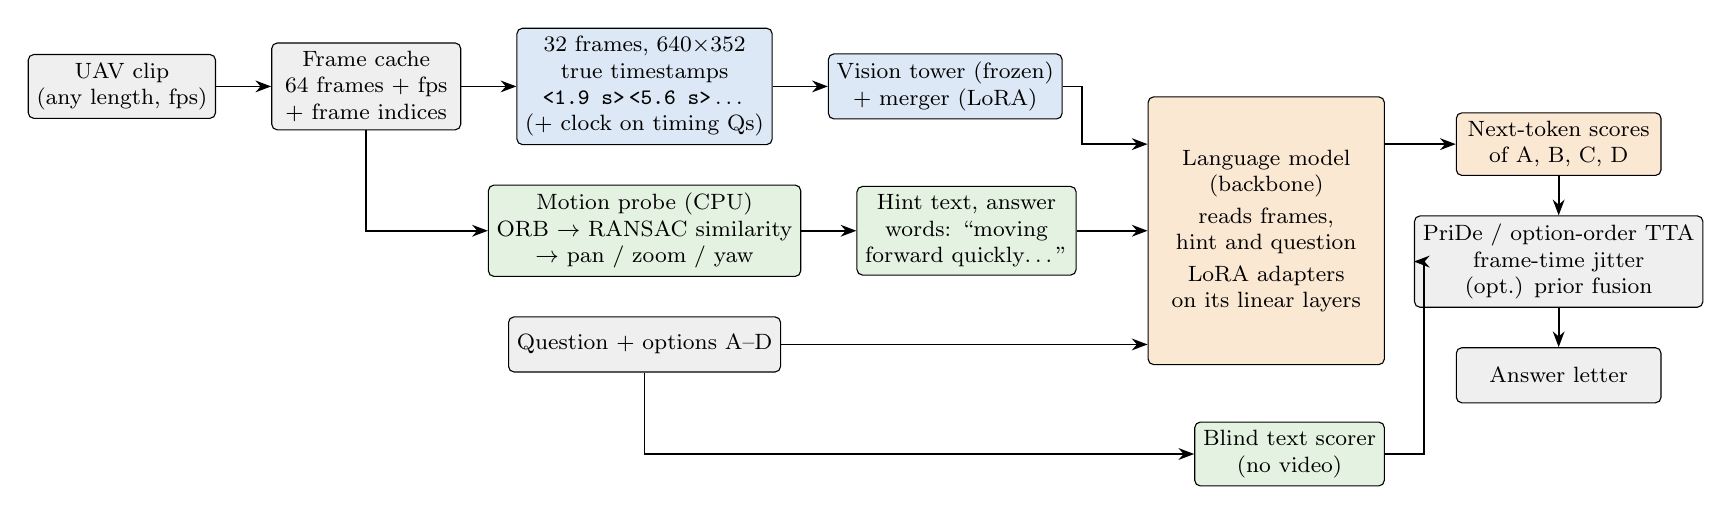
\begin{tikzpicture}[node distance=5mm and 7mm]
% lane 1: video
\node[box, fill=io, minimum width=21mm] (clip) {UAV clip\\(any length, fps)};
\node[box, fill=io, right=of clip, minimum width=24mm] (cache) {Frame cache\\64 frames + fps\\+ frame indices};
\node[box, fill=vis, right=of cache, minimum width=30mm] (frames) {32 frames, 640$\times$352\\true timestamps\\\texttt{<1.9 s>}\,\texttt{<5.6 s>}\,\ldots\\(+ clock on timing Qs)};
\node[box, fill=vis, right=of frames, minimum width=24mm] (vit) {Vision tower (frozen)\\+ merger (LoRA)};
% lane 2: cue
\node[box, fill=cue, below=of frames, minimum width=30mm] (probe) {Motion probe (CPU)\\ORB $\to$ RANSAC similarity\\$\to$ pan / zoom / yaw};
\node[box, fill=cue, right=of probe, minimum width=24mm] (text) {Hint text, answer\\words: ``moving\\forward quickly\ldots''};
% lane 3: question
\node[box, fill=io, below=of probe, minimum width=30mm] (qa) {Question + options A--D};
% language model spanning the lanes
\node[box, fill=llm, right=9mm of text, minimum width=30mm, minimum height=34mm] (lm) {Language model\\(backbone)\\[2pt]reads frames,\\hint and question\\[2pt]LoRA adapters\\on its linear layers};
% outputs
\node[box, fill=llm, right=9mm of lm, minimum width=26mm, yshift=11mm] (head) {Next-token scores\\of A, B, C, D};
\node[box, fill=io, below=of head, minimum width=26mm] (dec) {PriDe / option-order TTA\\frame-time jitter\\(opt.) prior fusion};
\node[box, fill=io, below=of dec, minimum width=26mm] (out) {Answer letter};
\node[box, fill=cue, left=9mm of out, minimum width=24mm, yshift=-10mm] (blind) {Blind text scorer\\(no video)};
% edges
\draw[arr] (clip) -- (cache);
\draw[arr] (cache) -- (frames);
\draw[arr] (cache.south) |- (probe.west);
\draw[arr] (frames) -- (vit);
\draw[arr] (probe) -- (text);
\draw[arr] (vit.east) -- ++(2.5mm,0) |- ([yshift=11mm]lm.west);
\draw[arr] (text.east) -- (lm.west |- text.east);
\draw[arr] (qa.east) -- (lm.west |- qa.east);
\draw[arr] (qa.south) |- (blind.west);
\draw[arr] (lm.east |- head.west) -- (head.west);
\draw[arr] (head) -- (dec);
\draw[arr] (blind.east) -- ++(5mm,0) |- (dec.west);
\draw[arr] (dec) -- (out);
\end{tikzpicture}}
\caption{The Peekaboo-VL pipeline. Each clip is decoded once into a cache
that keeps its frame rate and which frames were taken, so the prompt can
carry true times. A CPU step measures how the camera moves between frames
and writes it as one line of text in the answers' own words. The backbone
language model, fine-tuned with LoRA, scores the four letters. The final step can remove letter bias
and, optionally, mix in a text-only prior.}
\label{fig:system}
\end{figure*}


Drone video is an unfriendly input for a video language model. The camera
never stops moving, often faster than anything on the ground, so ``the car
moves'' and ``the camera moves'' look alike. The cars are a few pixels
wide. And many questions ask \emph{when} something happens, which needs a
finer sense of time than the model usually gets.

The ReVA benchmark~\cite{yao2026reva} tests exactly this, with eleven
question tasks over clips from VisDrone, UAVDT, ERA and a new collection,
Hawk-UAV. The organizers' own model, ReMoSense, extends
Qwen2.5-VL-7B~\cite{qwen25vl2025} with learned camera-motion tokens and
object tokens and reaches 80.04\% on test. Their ablation says the
camera-motion tokens alone are worth 3.9 points overall and 9 points on
temporal questions. So camera motion matters. The question is how to get it
into the model.

Training new motion modules was not an option for us. So we asked a
simpler question: if the model cannot see the camera motion well, why not
just tell it? Drone footage makes that cheap. The ground is far away and
close to flat, so how one frame lines up with the next is described by a
shift, a zoom and a rotation. Classic computer vision measures those in a
few milliseconds on a CPU. We write the result as one line of text and let
fine-tuning decide how much to trust it (Fig.~\ref{fig:system}). The same
idea covers two other things the model cannot easily see: the true time of
each frame, which recent Qwen models read as text
timestamps~\cite{qwen3vl2025}, and the habits of whoever wrote the
answers, which a tiny text-only model picks up surprisingly well.

We entered the ReVA challenge with one A40 GPU and a few weeks.
This paper reports what that budget bought, including the experiments
that failed. Our contributions are:

\begin{itemize}
\item \textbf{Tell, don't learn.} We inject camera ego-motion as text
instead of adding learned motion tokens. A CPU probe measures the motion
between sampled frames in a few milliseconds, and we render it in the
benchmark's own answer vocabulary (``moving forward'', ``panning left''),
so the model can match it to the options. Fine-tuned with LoRA on
Qwen3.5-9B, the system reaches 83.6\% on the ReVA test leaderboard, 3.5
points above the organizers' purpose-built ReMoSense-7B, using no new
network parts and one GPU. We are explicit about where this margin comes
from: the 9B backbone alone already matches ReMoSense, and fine-tuning on
the seen videos adds the rest. After fine-tuning, the model demonstrably
reads the hint, but removing it costs only about 0.2 points overall.
\item \textbf{A benchmark audit.} The ReVA test set asks new questions
about videos that are already in training, and the official validation set
is largely a copy of training questions. We build a development split with
no training-answer leak that mirrors the test regime and tracks the test
score to about one point. A fifth of it are test questions whose answers
the validation set happens to contain, and we say so. We argue that ReVA
results should be reported alongside a trained blind baseline and per-task
numbers.
\item \textbf{Wording over measurement.} The same motion measurements,
written in image terms (``the image shifts up'') rather than the answers'
words, \emph{lowered} a small model's accuracy on camera-motion questions
by 12.5 points; the answer words raised it by 16. A text hint's wording is
first-order, not a detail.
\item \textbf{An empirical map, negative results included.} We measure
what each part is worth with pre-registered success rules: the motion hint
after fine-tuning, question packing, letter-prior debiasing and prior
fusion, an object-motion hint, a caption hint from the benchmark's own
question writer, a second training epoch, and frame density at test
time. Temporal grounding stays the hardest task, and its errors are
near-misses of about one second---the gap between the timestamps the model
sees.
\end{itemize}

The rest of the paper follows the system: data and split
(Sec.~\ref{sec:data}), what it is built on and how it compares to prior
work (Sec.~\ref{sec:related}, Sec.~\ref{sec:background}), the method
step by step (Sec.~\ref{sec:method}), the main results
(Sec.~\ref{sec:results}), and an ablation of every part
(Sec.~\ref{sec:ablation}).

% Peekaboo-VL report: 02_related. Included from ../peekaboo_report.tex.
\section{Related Work}
\label{sec:related}

\textbf{Video language models.} Qwen2.5-VL~\cite{qwen25vl2025} tells the
model the time of each frame through the way it numbers token positions
(a ``rotary position'' scheme). Qwen3-VL~\cite{qwen3vl2025} replaces this
with plain text timestamps, such as ``\texttt{<3.0 seconds>}'', placed
before each pair of frames. Qwen3.5~\cite{qwen35} reuses the Qwen3-VL
vision part on a new language model. In that model, three out of every four
layers are ``Gated DeltaNet''~\cite{yang2025gdn} layers, which work like a
running memory and are cheaper than standard attention; every fourth layer
is standard attention. We build on Qwen3.5 and use its text timestamps as
one of the things we ``tell'' the model.

\textbf{Question answering on drone and remote-sensing video.}
ReVA~\cite{yao2026reva} introduces the benchmark and the ReMoSense model.
ReMoSense learns camera-motion tokens from cost volumes (a dense map of how
well each patch matches the next frame) and object tokens from a recurrent
transformer. Our motion hint carries the same kind of information, but as
text, with no new model parts. EgoSIS~\cite{yang2026egosis} is the closest
drone work we know of. It fits a robust image-plane transform between frames
from optical flow, which is almost the same measurement our probe makes, and
turns it into four learned ``spatial evidence'' tokens per slice of video on
top of Qwen3-VL. On SIS-Bench this lifts an 8B model from 63.1\% to 76.2\%.
So the two routes start from the same signal and differ only in how it
reaches the language model: as learned tokens, or as a sentence.
UrbanVideo-Bench~\cite{zhao2025urbanvideo}
is another drone-video benchmark. Its videos are filmed from a drone flying
through city streets, and its questions test whether a model can follow
the flight, remember what it saw, and plan. Its 5,355 multiple-choice
questions have between two and seven options. Unlike ReVA, it asks mainly
about the drone's own movement and route, which is close to our
camera-motion questions. We use it only as an outside test of whether our
motion hint carries over to other drone videos; we never train on it.

\textbf{Camera motion in video models.} CameraBench~\cite{lin2025camerabench}
shows that classic geometry methods (``structure from motion'') fail on
camera movements that need understanding of the scene, while video models
fail on simple geometric ones. Combining the two works better than either.
Feng et al.~\cite{feng2026geocam} look inside a Qwen2.5-VL vision encoder
and find that camera motion is only weakly represented, especially in its
later layers. They extract camera motion with a 3D geometry model, turn it
into motion labels with a small classifier, and give these labels to the
video model in the prompt. This improves camera-motion answers without
fine-tuning the video model. Their approach is the closest to ours: both
\emph{tell} the model the camera motion in text. Ours differs in three
ways. We use a much simpler and faster estimator, because drone scenes are
nearly flat. We write the hint in the exact words of the benchmark's
answers. And we fine-tune the model together with the hint, so it learns
when to trust it. Two recent papers learn the motion instead.
CameraVLM~\cite{cheng2026cameravlm} trains camera and optical-flow tokens
together with the language model and argues that the motion has to be read
by the language model, not estimated on its own. CamDistill~\cite{du2026camdistill}
distills the camera tokens of a 3D model into the video model during
training, so the 3D model is not needed at test time. It also tries our kind
of shortcut, writing the 3D model's per-frame pose as text in the prompt,
without fine-tuning. That helps the model find \emph{when} the motion
changes but not \emph{which} motion it is. Our results point at the wording
as one reason. Given to a small model without fine-tuning, the same motion
numbers dropped camera-motion accuracy from 68.2\% to 55.7\% when written in
image terms, and brought it to 71.6\% when written in the answers' words
(Sec.~\ref{sec:cue}). Our estimator itself uses ORB
features~\cite{rublee2011orb}, simple matching, and a RANSAC
fit~\cite{fischler1981ransac}.

\textbf{Biases in multiple-choice answers.} Language models prefer some
option letters regardless of the content, for example ``A'' over ``D''.
PriDe~\cite{zheng2024pride} measures this preference by showing the same
question with the options in rotated orders, and then divides it out,
without needing any correct answers. Ok et al.~\cite{ok2026optionbias}
split this kind of bias into two parts: how often an answer flips when the
options are reordered, and how strongly the answers lean toward some
letters. Prior correction such as PriDe mostly fixes the lean, while
averaging over option orders mostly reduces the flips. We use both: PriDe
and option shuffling at test time, and random option order during training.

A related, older problem is the \emph{language prior}: patterns in the
questions and answers that reveal the answer without the image. Goyal et
al.~\cite{goyal2017vqav2} showed how strong such priors were in image
question answering, and Chakraborty et al.~\cite{chakraborty2026visualoptions}
show that video models still lean on the wording of text options: one strong
model drops from about 74\% to about 30\% when the same options are shown as
frames instead. For aerial video in particular, a recent meta-analysis of 67
papers~\cite{angelidis2026aerialgap} found that none of the aerial
question-answering benchmarks reports a blind (text-only) score, so there is
no floor to read their accuracies against. Our trained blind baseline
(Sec.~\ref{sec:blind}) gives that floor for ReVA.

% Peekaboo-VL report: 03_data. Included from ../peekaboo_report.tex.
\section{Task and Data}
\label{sec:data}

\subsection{The benchmark}
Each ReVA record has a video path, a question, four options (A--D) and, for
training data, the correct letter. The questions fall into eleven tasks in
four groups (Table~\ref{tab:tasks}). The challenge test set has 4,000
questions over 1,014 clips. The score is accuracy, overall and per task.
Fig.~\ref{fig:sample} shows one training clip with three of its questions,
and Fig.~\ref{fig:gallery} shows one question from each video source.

\begin{figure*}[t]
\centering
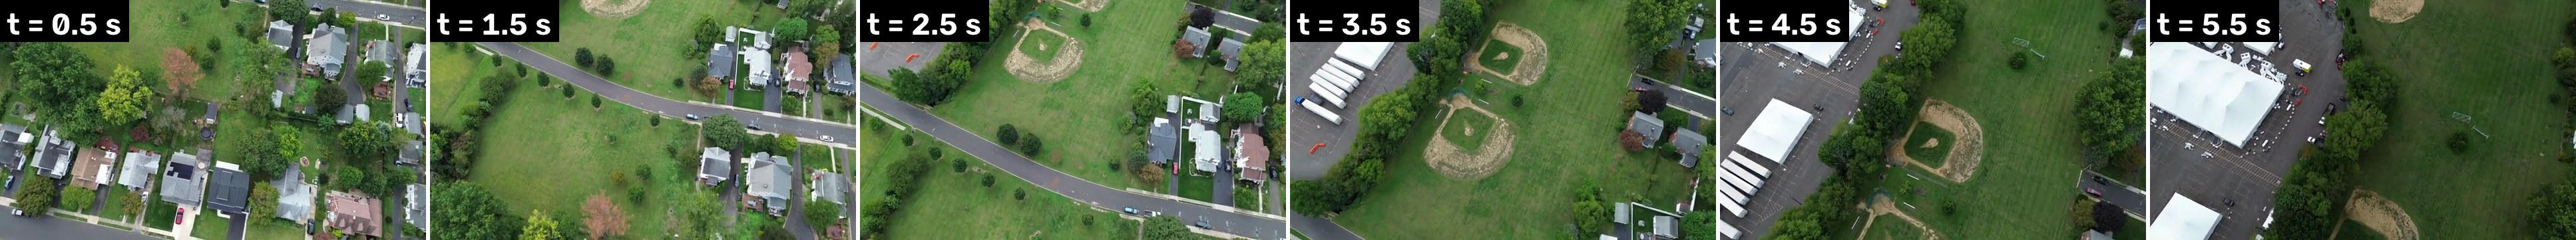
\includegraphics[width=\textwidth]{figures/sample_frames.jpg}\\[3pt]
\footnotesize
\begin{tabular}{@{}p{0.11\textwidth}p{0.42\textwidth}p{0.40\textwidth}@{}}
\toprule
Task & Question & Options (correct one in bold) \\
\midrule
TU\_Temporal & At what point in the video do the white tents first appear in the frame? &
A.~4.8\,s \quad \textbf{B.~3.5\,s} \quad C.~2.0\,s \quad D.~0.0\,s \\
SR\_Viewpoint & What is the primary camera motion state throughout the video? &
A.~Panning left/right \quad \textbf{B.~Moving forward} \quad C.~Zooming in/out \quad D.~Rotating \\
FP\_Change & How does the camera's perspective change throughout the video? &
\textbf{D.~From a wide aerial view of the neighborhood to a closer view of the field and tents} (3 other options) \\
\midrule
\multicolumn{3}{@{}l@{}}{\textit{Our motion hint for this clip:} ``Camera motion: 0.1--5.9s moving
forward quickly while rotating clockwise. Mostly moving forward (100\% of the clip).''} \\
\bottomrule
\end{tabular}
\caption{A ReVA training clip (\texttt{Hawk\_UAV/PH/DJI\_0229\_d4\_01}):
six evenly spaced frames with their true times, three of its questions, and
the motion hint our system writes for it. The tents enter the frame at
$t{=}3.5$\,s, which is the answer to the temporal question. The hint
already contains the answer to the camera-motion question, in the option's
own words.}
\label{fig:sample}
\end{figure*}


\begin{figure*}[t]
\centering
\footnotesize
\setlength{\tabcolsep}{3pt}
\resizebox{\textwidth}{!}{%
\begin{tabular}{@{}c@{\hspace{6pt}}c@{}}
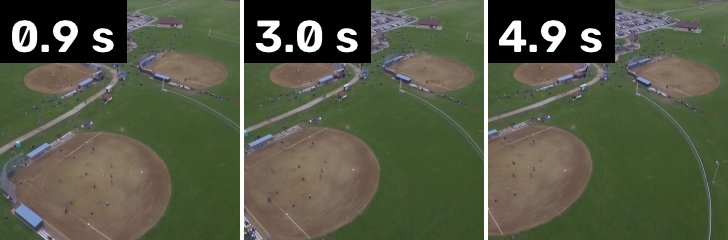
\includegraphics[height=19mm]{figures/gallery_era.jpg} &
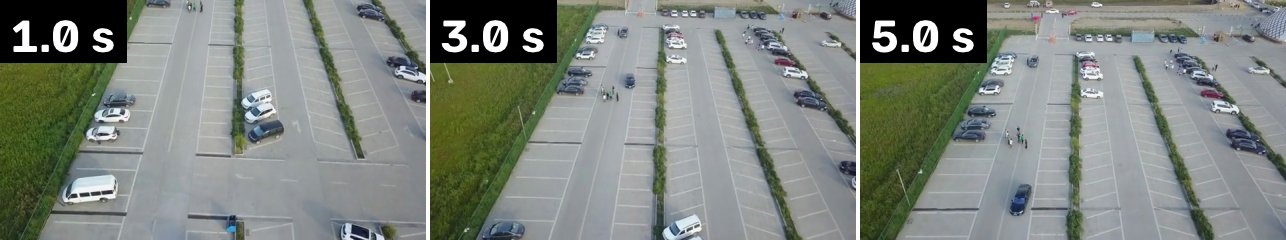
\includegraphics[height=19mm]{figures/gallery_visdrone.jpg} \\[1pt]
\parbox[t]{0.31\textwidth}{\textbf{ERA, CR\_Causation.} Likely cause of the many parked cars?
\textbf{(B) Baseball games} (vs.\ restaurant, highway, mall).} &
\parbox[t]{0.55\textwidth}{\textbf{VisDrone, FP\_ObjectLand.} What type of land cover is visible on
the left side of the parking lot? (A) A paved road \ (B) A body of water \ (C) A dense forest \
\textbf{(D) A field of green grass}.} \\[20pt]
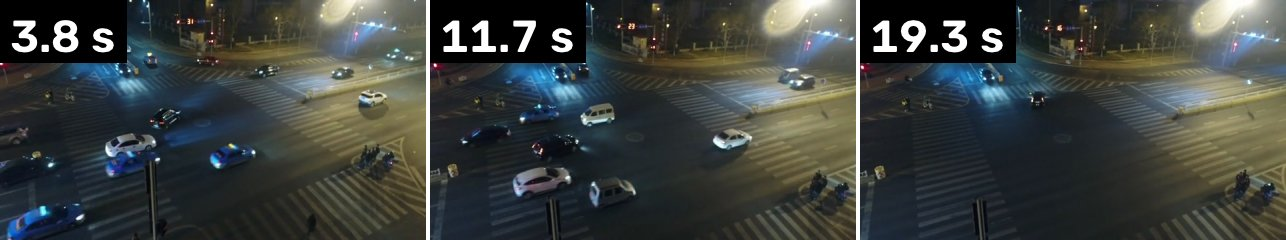
\includegraphics[height=16mm]{figures/gallery_uavdt.jpg} &
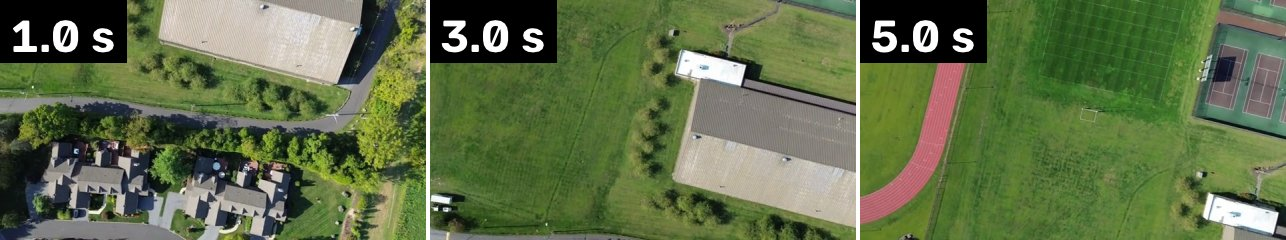
\includegraphics[height=16mm]{figures/gallery_hawk.jpg} \\[1pt]
\parbox[t]{0.46\textwidth}{\textbf{UAVDT, TU\_Temporal} (23.2\,s clip). At what time does the white
van first appear in the video? (A) 0:08 \ (B) 0:12 \ \textbf{(C) 0:03} \ (D) 0:05.} &
\parbox[t]{0.46\textwidth}{\textbf{Hawk-UAV, SR\_Geometric.} How is the tennis court positioned
relative to the soccer field? (A) Above \ (B) To the left \ (C) Below \ \textbf{(D) To the right}.} \\
\end{tabular}}
\caption{One example from each of the four video sources, three evenly spaced frames each with
their true times (correct answers in bold). ERA clips are square and about 6\,s long; UAVDT clips
can last tens of seconds; temporal questions use both seconds and \texttt{m:ss} formats.}
\label{fig:gallery}
\end{figure*}

\begin{table}[t]
\centering
\caption{The eleven tasks and how many test questions each has.}
\label{tab:tasks}
\footnotesize
\begin{tabular}{@{}llr@{}}
\toprule
Group & Task (leaderboard name) & Test Q \\
\midrule
\multirow{3}{*}{Factual Perception} & General Understanding (FP\_General) & 180 \\
 & Object \& Land Cover (FP\_ObjectLand) & 660 \\
 & Change Detection (FP\_Change) & 500 \\
\midrule
\multirow{2}{*}{Temporal} & Temporal Grounding (TU\_Temporal) & 640 \\
 & Trend \& Pattern (TU\_TrendPattern) & 360 \\
\midrule
\multirow{3}{*}{Spatial} & Geometric Relation (SR\_Geometric) & 400 \\
 & Structural Layout (SR\_Structural) & 340 \\
 & Perspective \& Viewpoint (SR\_Viewpoint) & 480 \\
\midrule
\multirow{3}{*}{Causal} & Causation (CR\_Causation) & 180 \\
 & Consequence (CR\_Consequence) & 100 \\
 & Hypothetical (CR\_Hypothetical) & 160 \\
\bottomrule
\end{tabular}
\end{table}

\textbf{What the tasks ask, in plain words.}
\emph{General Understanding} asks what the video is about or what is in it.
\emph{Object \& Land Cover} asks what kinds of objects or ground (grass,
water, buildings) appear, and sometimes how many. \emph{Change Detection}
asks how something changes during the clip, such as how a car moves or how
the view changes. \emph{Temporal Grounding} asks when something happens, as
a time or a time range. \emph{Trend \& Pattern} asks about repeated or
overall movement, such as the main direction of traffic. The three spatial
tasks ask where things are relative to each other, how the area is laid
out (for example, a grid of roads), and how the camera looks at or moves
over the scene. The three causal tasks ask why something happens, what will
happen next, and what would happen if something were different. These last
three rely mostly on general knowledge and are already easy for large
models.

\subsection{What the data files reveal: same videos, new questions}
Before building anything, we checked the released files carefully.
Table~\ref{tab:audit} summarizes what we found.

The most important fact is this: 1,012 of the 1,014 test clips, and all 529
longer source videos they were cut from, also appear in the training set.
3,997 of the 4,000 test questions are about a clip that has training
questions. But the test questions themselves are new. Only 24 are exact
copies of a training question on the same clip, and 334 are close copies
(at least 60\% of their words in common). So the test asks \emph{new
questions about videos the model has already seen in training}.

The official validation set is different. 1,572 of its 2,000 questions
repeat a training question on the same clip, and 1,569 of those have the
same answer. A model trained on the training set will look good on
this validation set simply because it remembers the answers. That number
would tell us little about the test.

\begin{table}[t]
\centering
\caption{What the released annotation files show.}
\label{tab:audit}
\footnotesize
\begin{tabular}{@{}lr@{}}
\toprule
Statistic & Value \\
\midrule
Train / val / test questions & 15,773 / 2,000 / 4,000 \\
Train / val / test clips & 1,045 / 379 / 1,014 \\
Test clips also in train & 1,012 / 1,014 \\
Test questions on train clips & 3,997 / 4,000 \\
Test exact copies of train questions & 24 \\
Test close copies (word overlap $\geq 0.6$ / $\geq 0.8$) & 334 / 67 \\
Val exact copies of train questions & 1,572 / 2,000 \\
Correct answer is the longest option (train+val) & 36.3\% \\
\midrule
Our fit / dev split (questions) & 14,068 / 2,078 \\
Dev questions on fit clips & 2,074 / 2,078 \\
\bottomrule
\end{tabular}
\end{table}

\subsection{A development split that behaves like the test}
Because the official validation set cannot be trusted, we built our own
split. Our \emph{dev} set has two parts: the 428 validation questions that
are \emph{not} copies of training questions, and 150 randomly chosen
training questions per task, set aside. Our \emph{fit} set (the data we
train on) is everything else, after removing every record that asks a dev
question about the same clip. The clips are still shared between fit and
dev, just as they are shared between train and test. This copies the
``same video, new question'' setting of the real test.

One property of this split must be stated plainly. The 428 validation
questions that are not copies of training questions turn out to be copies
of \emph{test} questions: all 428 have the same clip and the same question
text as a test question. So 20.6\% of dev are test questions whose answers
the official validation file contains. They are not training answers, so
dev has no training-answer leak, but dev is not disjoint from the test,
and its agreement with the test score is partly built in. The other 1,650
dev questions are held-out training questions.

The dev set has 2,078 questions. With that many questions, the accuracy has
a margin of error of about $\pm 0.9$ points. Dev tracks the test well: our
blind scorer gets 55.5\% on dev and 55.9\% on the test leaderboard, and the
test-weighted dev accuracy (below) lands within 0.2 points of the test for
our first fine-tuned model and within about 1.2 points for the final one
(Sec.~\ref{sec:results}).

One more detail matters. The tasks do not have the same share of questions
in dev and in test. Dev has 150--231 questions per task, while the test has
100 to 660. Some tasks that are common in the test, such as Temporal
Grounding (640 questions), are among the hardest. So we also compute a
\emph{test-weighted} dev accuracy, where each task's dev accuracy is
weighted by its number of test questions. This is the number we use to
pick between systems.

\subsection{The clips are not all alike}
The dataset card describes 15-second clips at 640$\times$360 pixels.
Decoding all 1,047 clips used by the questions shows a different picture
(Table~\ref{tab:clips}). ERA clips are square and under 6\,s. Hawk-UAV
clips range from 0.1 to 40\,s. Ten clips are shorter than one second, yet
they carry 137 questions between them; those questions cannot be answered
from the video. Because we always show the model the same number of frames
(16 in our first runs, 32 in the final model), the time between two frames
ranges from a fraction of a second to more than two seconds. This is why the model must be told the \emph{true} time of each
frame, computed from each clip's own frame rate.

\begin{table}[t]
\centering
\caption{Clips used by the questions, by source (decoded from the released files).}
\label{tab:clips}
\footnotesize
\begin{tabular}{@{}lrcrc@{}}
\toprule
Source & Clips & Res. & fps & Length (s) min/med/max \\
\midrule
Hawk-UAV & 556 & 640$\times$360 & 30 & 0.1 / 8.0 / 40.2 \\
ERA~\cite{mou2020era} & 261 & 640$\times$640 & $\sim$24 & 5.4 / 5.8 / 5.8 \\
VisDrone~\cite{zhu2021visdrone} & 183 & 640$\times$360 & 30 & 0.2 / 6.0 / 6.0 \\
UAVDT~\cite{du2018uavdt} & 47 & 640$\times$360 & 30 & 3.9 / 16.0 / 35.0 \\
\bottomrule
\end{tabular}
\end{table}

\subsection{Training data balance}
The task mix of the training data differs from the test. Temporal
Grounding and Object \& Land Cover are 12.2\% and 11.1\% of our fit set,
but 16.0\% and 16.5\% of the test. Both are weak tasks for our model. This
suggests giving these tasks more weight during training, which is one of
the next experiments.

% Peekaboo-VL paper: 04_background. Included from ../peekaboo_report.tex.
\section{Background}
\label{sec:background}

A video language model does not watch a whole clip. It reads a small number
of frames, 16 or 32 in this paper, taken at even intervals. Each frame is cut into patches,
a vision encoder turns the patches into vectors, and the vectors are placed
into the language model's input next to the words of the question.
Qwen3-VL and Qwen3.5 also write a short text timestamp (for example
\texttt{<3.0 seconds>}) before each pair of frames, which is how the model
knows \emph{when} each frame was taken.

This design has two weak points on drone video. The motion between frames is
never given directly: the model must infer it from differences between frames
that may be a second apart. And with 16 frames the model sees roughly one
timestamp per second on a typical clip (two per second at 32), so it cannot separate events closer together than
that. The rest of the paper addresses both.

Our remaining design choices are standard, so we fix them here and use them
throughout. We score the four answer letters instead of generating an
answer (Sec.~\ref{sec:method}). We fine-tune with
LoRA~\cite{hu2022lora}. We measure the video's true contribution against a
blind text-only baseline (Sec.~\ref{sec:blind}), following the lesson of
Goyal et al.~\cite{goyal2017vqav2} that question sets carry answer patterns
which need no image. And we compare two systems with a paired exact McNemar
test, under success rules written down before each run.

% Peekaboo-VL report: 05_method. Included from ../peekaboo_report.tex.
\section{Method}
\label{sec:method}

Fig.~\ref{fig:system} shows the whole pipeline. We explain it in the order
in which a question goes through it.


\subsection{Step 1: decode each clip once}
Decoding video is the slowest part of reading it, and each clip is used by
about 15 questions. So each clip is decoded once into a cache of 64 evenly
spaced frames. For all 1,047 clips this takes under a minute and about
7\,GB of disk; after that, loading a clip's frames is a plain file read. Together
with the frames we store the clip's frame rate and the exact frame numbers
we took. From these, the true time of every frame is known. The final
model takes 32 of the 64 frames (our first runs used 16). Each frame comes
from one of 32 equal time segments, a standard choice from action
recognition~\cite{wang2016tsn}. A ``phase'' setting decides where inside
its segment a frame is taken. At test time we take the centre. During
training we draw a new random phase for every question, so the model sees
many different sets of timestamps for the same clip. A model trained on one
fixed set of frames gets worse when the frames shift
(Sec.~\ref{sec:ablation}); random phases remove that weakness, and they act
as a small data augmentation as well.

\subsection{Step 2: two processor defaults that silently hurt}
Two default settings in the Qwen3.5 video processor would have hurt us.
Neither raises an error or a warning; we only found them by reading the
prompt the processor actually builds.

\emph{Image size.} The processor has a pixel budget
(\texttt{size.longest\_edge}, default 786,432 pixels). This budget covers
\emph{all} frames together, not each frame. With 32 frames, it would shrink
each 640$\times$360 frame to about 208$\times$117 pixels, where a car is
just a few pixels. We scale the budget with the number of frames, so each
frame stays at 640$\times$352. This gives 220 visual tokens for each pair
of frames, about 3,500 for the 32 frames of a clip.

\emph{Timestamps.} The processor computes frame times from video metadata.
When frames are given without that metadata, it assumes 24 frames per
second, so the times written in the prompt are wrong. Our cache passes the
true frame rate and frame numbers. We checked the final prompt for a
25\,fps, 15\,s clip and it contains the correct
\texttt{<1.9/5.6/9.3/13.1 seconds>} labels.

\subsection{Step 3: measure the camera motion}
For each pair of neighbouring sampled frames we do the following
(Fig.~\ref{fig:probe}).
\begin{enumerate}
\item Find a few hundred distinctive points (ORB
keypoints~\cite{rublee2011orb}) in both frames, such as road markings and
roof corners.
\item Match points between the two frames. A ``ratio test'' throws away
matches that are not clearly better than the second-best choice.
\item Fit one transform that explains most matches: a shift, a zoom and a
rotation (a ``similarity'' transform with four numbers). RANSAC
\cite{fischler1981ransac} handles the outliers: it tries many small random
sets of matches and keeps the transform that agrees with the most of them.
Matches on moving cars do not agree with the ground, so they are ignored.
\item Turn the four numbers into a label. The camera moves opposite to the
scene: if the ground slides to the left, the camera is panning right. A
camera tilted forward and flying forward sees the ground slide down and
grow larger. Rotation means the camera turns. Small numbers mean the camera
is still.
\end{enumerate}
We then join neighbouring steps with the same label into timed segments,
and fold segments shorter than 0.8\,s into a neighbour. The whole probe
takes a few milliseconds per frame pair on one CPU core; all 1,047 clips
take under a minute.

Why not a learned motion model? Because this one needs no training, no GPU
time and no labels, and its output is a sentence we can read and check.
When it is wrong, we can see why (Sec.~\ref{sec:results} shows where it
fails).

\begin{figure}[t]
\centering
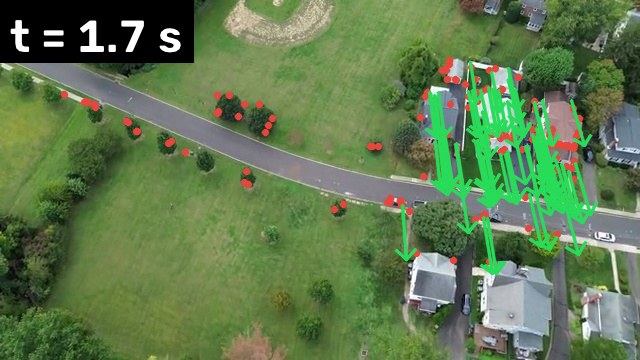
\includegraphics[width=0.92\columnwidth]{figures/probe_tracks.jpg}
\caption{The motion probe between two sampled frames of the clip in
Fig.~\ref{fig:sample}. 304 of 450 point matches agree with one transform
(green, 80 shown at random). They all stream downward, which is what
forward flight looks like. Red dots are rejected matches, here on trees
whose leaves all look alike.}
\label{fig:probe}
\end{figure}

\subsection{Step 4: write the motion in the answers' words}
The first version of the hint described what happens \emph{in the image}:
``pans toward the top of the frame, fast and zooms in (descending)''.
Section~\ref{sec:cue} shows that this wording confused the model. The final
version uses the words of ReVA's camera-motion answers: \emph{moving
forward / backward}, \emph{panning left / right}, \emph{rotating},
\emph{stationary}, with a speed word and a short summary at the end, for
example:

\smallskip
\noindent\fbox{\parbox{0.95\columnwidth}{\footnotesize\ttfamily
Camera motion: 0.1-5.9s moving forward quickly while rotating clockwise.
Mostly moving forward (100\% of the clip).}}
\smallskip

\subsection{Step 4b: a second hint, counts from a detector}
\label{sec:counts}
The camera hint says how the \emph{camera} moves, not how many objects are
in the scene. Video models are known to undercount small, dense objects, and
``Object \& Land Cover'' is one of ReVA's largest tasks. We therefore add a
second hint produced by a VisDrone-trained detector (YOLO11x), the only
learned component in the pipeline besides the model itself. The detector
runs on the first, middle and last of the clip's cached frames, and its
counts are merged into the words the questions use (``person'', ``car'',
``truck'') and written as one sentence:

\smallskip
\noindent\fbox{\parbox{0.95\columnwidth}{\footnotesize\ttfamily
Detector counts: 0.0s car 23, pedestrian 4, truck 2; 3.0s car 19; 5.9s car
31, truck 3.}}
\smallskip

ReVA's counting answers are ranges (``10--20''), so a detector error of
about 20\% usually still lands in the correct range. The counts are
computed once for all 1,047 clips and stored next to the motion hints, so
training and testing add no detector cost. We built the hint for every
clip but did not get to evaluate it within our compute budget, so the
final model does not use it.

\subsection{Step 4c: a clock drawn on the frames of timing questions}
\label{sec:timebar}
The timestamps in the prompt tell the model \emph{when} each frame was
taken, but only as text next to the frames. Temporal Grounding questions ask
exactly this (``At what time does the red car first appear?''), and they
are our weakest task. Following VTimeCoT~\cite{zhang2025vtimecot}, we also
\emph{draw} the time on the frames: a dark strip along the bottom edge, a
red bar that fills from left to right as the clip plays, and the frame's
time in seconds (``3.5s''). The model can then read the time from the image
itself.

We draw the bar only for Temporal Grounding questions. Drawing it on every
question helped timing questions but cost object questions, because the
strip covers the bottom 16 pixels of the frame, where small cars and people
often are. The bar is drawn the same way in training and in testing, so the
model learns to use it. Tested on a model that was trained without it, the
bar already raised Temporal Grounding by 0.9 points on dev.

\subsection{Step 5: build the prompt}
The model receives one user message: the 32 frames with their timestamps
(with the drawn clock for Temporal Grounding questions), then the hint line,
the question, the four options and a fixed instruction.
Qwen3.5 can ``think'' in
writing before answering; we switch this off, so the answer letter comes
right after the start of the model's reply.

\subsection{Step 6: score the four letters}
At the answer position we read the model's scores (logits) for the tokens
A, B, C and D and treat them as the scores of four classes. To save memory,
we compute scores only for that one position. During training, the loss is
the usual cross-entropy over these four scores. In other words, we train
the model to put high probability on the correct letter, and we ignore all
other words. There is no text generation and no answer parsing.

We chose this over generating an answer for three reasons. It never fails
to produce a valid letter. It gives four scores per question, which the
later steps (letter debiasing, mixing in a prior, combining models) need.
And it is cheap: computing scores only for the last position avoids
building the full 250k-word output layer for every token. Scoring takes
0.63\,s per question on the A40 at 16 frames and about 1.4\,s at 32 frames
(Step~7b makes this faster).

\subsection{Step 7: fine-tune with LoRA}
We attach LoRA adapters~\cite{hu2022lora} (rank $r{=}64$, scale
$\alpha{=}128$, dropout 0.05) to every linear layer of the language model.
This covers the attention layers, the Gated DeltaNet layers and the
feed-forward layers. We also attach them to the small ``merger'' that
connects the vision part to the language part. The vision encoder itself
stays frozen. In total, 161.6M of 9.57B parameters are trained (1.69\%).
The adapter file is about 620\,MB, so keeping many experiments around is
cheap, and training at 32 frames fits in 28\,GB of the A40's 46\,GB.

The final model trains on all 14,068 fit questions for one pass, with one
question per sequence. A second pass did not help: with branching
(Step~7b) and the learning rate decayed over two passes, the two-pass model
ends at 82.96\% test-weighted dev, against 83.04\% for one pass. A faster recipe packs eight questions about one clip
into one sequence (Sec.~\ref{sec:packing}). Packing costs accuracy, and we
now know why: each later question in the sequence can see the correct
answers to the earlier ones. The model therefore trains on a prompt it never
sees at test time, and with packing, more training data did not help.
Step~7b gives the speed of packing without this leak.

Every time a training question is used, we shuffle its four options into a
new random order. The correct answer is therefore equally likely to be A,
B, C or D, and the model cannot learn to prefer a letter.
Table~\ref{tab:setup} lists all settings of the main run.

\begin{table}[t]
\centering
\caption{Training and test settings of the final model (H20).}
\label{tab:setup}
\footnotesize
\begin{tabular}{@{}ll@{}}
\toprule
Base model & Qwen3.5-9B, bf16, SDPA attention \\
Video input & 32 frames, 640$\times$352, true timestamps \\
Frame sampling & random phase per question (train), centre (test) \\
Hints & camera motion, in answer words; \\
 & drawn clock on Temporal Grounding frames \\
Adapter & LoRA $r{=}64$, $\alpha{=}128$, LM linears + merger \\
Data & all 14,068 fit questions, one per sequence \\
Optimizer & AdamW, lr $10^{-4}$, 3\% warm-up, cosine decay \\
Batch & 1 $\times$ 16 accumulation, 880 steps (1 pass), clip 1.0 \\
Training time & 17\,h (about 70\,s per 16-question step) \\
Hardware & 1$\times$ NVIDIA A40 (46\,GB), 28\,GB used \\
Speed & 4.3\,s per training question \\
Decoding & PriDe~\cite{zheng2024pride} (5\% subset) or plain \\
\bottomrule
\end{tabular}
\end{table}

\subsection{Step 7b: one video pass for many questions, without leaks}
\label{sec:branch}
Each clip has about 15 questions, and the video makes up almost all of the
prompt (about 3,500 of 3,700 tokens). Scoring the questions one by one
therefore processes the same video 15 times. We split each prompt into a
\emph{prefix} shared by all questions about the clip (the video and the hint)
and a short \emph{suffix} per question (the question, the options and the
start of the answer). The prefix runs through the model once, and every
suffix then continues from it on its own branch:
\begin{itemize}
\item In the full-attention layers, each suffix attends to the prefix and to
its own earlier tokens, never to another suffix.
\item In the Gated DeltaNet layers, which keep a running state instead of
attending, each suffix starts from the state the prefix ends in (and from
the last few inputs of the layer's short convolution).
\end{itemize}
Every question therefore sees exactly the prompt it would see alone, so
nothing leaks between questions, and during training the gradients of all
branches add up in the shared prefix. We checked this against scoring the
questions one at a time on Qwen3.5-0.8B in 32-bit floats: the letter scores
agree to $10^{-4}$ and the adapter gradients to a relative $6\times10^{-5}$.
In 16-bit floats the scores move by rounding only. Scoring eight questions
per video pass was 3.7 times faster in our test, and the same split makes
training about as fast as packing. Questions with and without the drawn clock
see different frames, so they go into separate groups.

\subsection{Step 7c: two more training signals (being tested)}
\label{sec:extra-losses}
Both signals change only the training loss; the test prompt stays the same.

\emph{The clip played backwards.} Video models often give the same answer
when the frames are shuffled or reversed, which means they answer from what
is in the frames, not from their order~\cite{kang2026bpo}. For questions
whose answer must change when time runs backwards, we also show the model
the reversed clip and push it away from the original answer. These are
Temporal Grounding questions about a moment (``when does the bus first
appear''), Change Detection questions about a direction or a change, and
camera-motion questions (``moving forward''). Questions whose answer stays
the same, such as durations, a stationary camera or the viewing angle, are
left out by simple text rules; about 16\% of the fit questions qualify. The
reversed clip keeps its timestamps and clock running forward, and it gets
no motion hint, because the hint describes the original direction. With
$p_{\text{rev}}(y)$ the probability of the original answer $y$ on the
reversed clip, the loss becomes
\[
\mathcal{L} = \mathrm{CE} + \lambda_{\text{rev}}\,
\bigl(-\log\,(1 - p_{\text{rev}}(y))\bigr),\qquad \lambda_{\text{rev}} = 0.5 .
\]
The extra term only says ``not this answer''; it does not name a new one,
and it fades once the original answer is unlikely. Before spending a run on
it, we test whether the trained model already changes its answers on
reversed clips; if it does, this signal has little to teach.

\emph{The clip's facts as plain text.} The test set asks new questions about
clips the model has already trained on. In language models, facts learned
in a single format are often not recalled when the question is asked in a
new way; training on the same facts in two formats at once fixes much of
this~\cite{zhang2025factrecall}. Our training uses one format only: pick a
letter for four given options. So each group of questions about a clip gets
one extra branch (Step~7b) in which the model writes out that clip's
training questions with their answers as plain text, without options or
letters (``Q: When does the red car first appear? A: At 3.5 seconds''). The
pairs are shuffled every time and capped at 24. The loss adds
$\lambda_{\text{fact}} = 0.3$ times the mean word-level cross-entropy of this
text. Because the text branch is a separate branch, the letter questions
never see it; we checked that their scores are identical with and without
it. Dev questions never appear in the text.

\emph{Outcome.} The reversed-clip check ran first, on the final model's
dev answers: on the 375 questions whose answer should change, the model
kept its answer on the reversed clip 68.3\% of the time, against 88.0\% on
266 control questions whose answer should not change. The model already
uses frame order where it matters, so by our pre-registered rule (a gap
below 0.15 would justify the run; it is 0.197) we did not train with this
signal. The fact-text signal was built and checked but not trained within
our budget.

\subsection{Step 8 (optional): remove letter bias and mix in a text prior}
\label{sec:blind}
\emph{Letter bias.} PriDe~\cite{zheng2024pride} estimates how much the
model prefers each letter by scoring a small part of the test set with the
options rotated. It then divides this preference out of every score. It
needs no correct answers.

\emph{Blind prior.} We also train a small text-only scorer that never sees
the video. For each option it computes 50 simple features: how long the
option is compared with the others, how often similar answer texts were
correct in training for this task, how many words it shares with the
question, whether it is the largest or smallest number among the options,
and a few task-specific copies of the strongest features. A logistic model
over the four options learns how to weigh these features. It trains in
seconds. At test time we can combine it with the video model as
$\log p = \log p_{\text{VLM}} + \alpha \log p_{\text{blind}}$, where
$\alpha$ controls how much we trust the blind scorer. We choose $\alpha$ on
dev with cross-validation, with the folds split by clip so no clip is in
both halves.

\emph{Plain decoding.} Because the options are shuffled in training, the
fine-tuned model has almost no letter preference left, so PriDe has little
to correct. We therefore also tried plain scores: one pass with the official
option order and no correction. On dev the plain scores looked slightly
better, but on the test set PriDe won (83.55\% vs.\ 83.25\%). The plain
answers lean slightly towards ``A'' (26.9\% of answers), which is exactly
what PriDe removes. We keep PriDe. A dev difference below about one point
between two decodings of the same model is not a reliable guide.

\emph{Averaging over frame phases.} Shifting all frames by half a segment
changes about one answer in five on video benchmarks while leaving accuracy
unchanged~\cite{zhu2026phase}. A model trained with random phases (Step~1)
can be scored at several phases, for example 0.17, 0.5 and 0.83, and its
answer probabilities averaged. This removes the dependence on one phase at
the cost of one scoring pass per phase. We implemented it but did not
evaluate it; the submitted system scores the centre phase only.

% Peekaboo-VL report: 06_results. Included from ../peekaboo_report.tex.
\section{Results}
\label{sec:results}

\subsection{Experimental protocol}
Unless stated otherwise, we report accuracy on our development split
(Sec.~\ref{sec:data}), which mirrors the challenge's ``seen video, new
question'' test regime. Because dev's task mix differs from the test's, we
also report a \emph{test-weighted} accuracy that reweights the eleven tasks
by their test question counts. It predicted the leaderboard within 0.2
points for our first model and within about 1.2 points for the final one,
and it is our model-selection metric. Comparisons between two systems
use a paired exact McNemar test over the questions the two answer
differently. Each configuration is a single run at seed 42: we did not have
the budget for repeated seeds, so our claims rest on paired tests and on
decision rules written down before the run, not on seed averaging. All
models are Qwen3.5-9B in bfloat16 with LoRA adapter weights on the language
model and the vision--language merger (161.6M of 9.57B parameters, 1.69\%);
training runs on one NVIDIA A40 (46\,GB). Decoding is either the official
option order, the four cyclic option permutations averaged (4$\times$ the
cost), or PriDe debiasing~\cite{zheng2024pride} (Sec.~\ref{sec:blind}). We
report failed experiments alongside successful ones. Two systems appear
below: our \emph{first model} (16 frames, 8,000 fit questions), which was
our first leaderboard entry and the reference for most ablations, and the
final \emph{Peekaboo-VL} model (32 frames with random training phases, the
drawn clock on timing questions, all 14,068 fit questions;
Table~\ref{tab:setup}). Recall that 428 dev questions are test questions
(Sec.~\ref{sec:data}).

\subsection{How far do you get without the video?}
Table~\ref{tab:main} shows the main steps, from guessing to our final
system. Without any video, the blind scorer reaches 55.5\% on dev and
55.9\% on the test leaderboard. That is more than double random guessing:
over half of ReVA can be answered without looking at a single frame.
Without any fine-tuning, Qwen3.5-9B already reaches 79.6\% on dev, about the
same as ReMoSense after its full fine-tuning (80.0\% on test).

\begin{table}[t]
\centering
\caption{Overall accuracy (\%). Dev unless marked; ReMoSense numbers are
from its paper (test set).}
\label{tab:main}
\footnotesize
\begin{tabular}{@{}lrr@{}}
\toprule
System & Dev & Test \\
\midrule
Random guessing & 25.0 & 25.2 \\
Longest option / answer-text prior & 41.3 / 40.7 & -- \\
Blind text scorer (ours) & 55.5 & 55.9 \\
\midrule
Qwen3.5-0.8B, no fine-tuning$^\dagger$ & 71.6 & -- \\
\quad + blind prior ($\alpha{=}0.75$ fixed)$^\dagger$ & 77.6 & -- \\
Qwen3.5-4B, no fine-tuning & 77.0 & -- \\
Qwen3.5-9B, no fine-tuning & 79.6 & -- \\
\quad + blind prior ($\alpha$ by cross-validation) & 80.1 & -- \\
\midrule
ReMoSense-7B, fine-tuned~\cite{yao2026reva} & -- & 80.0 \\
First model (16 frames, 8k questions) + PriDe & 84.7 & 82.6 \\
\quad + blind prior ($\alpha$ by cross-validation, not used) & 85.2 & -- \\
\textbf{Peekaboo-VL} (32 frames, clock, all fit), plain & \textbf{85.4} & 83.3 \\
\quad + PriDe letter debiasing (submitted) & 85.0 & \textbf{83.6} \\
\bottomrule
\multicolumn{3}{@{}l@{}}{\scriptsize $^\dagger$On a 250-question dev subset (25 per task, no Viewpoint).}
\end{tabular}
\end{table}


\subsection{Which tasks are still hard?}
Fig.~\ref{fig:pertask} and Table~\ref{tab:pertask} compare the tasks.

The blind scorer does best where the same answers come up again and again:
Viewpoint (72\% on both dev and test) and General Understanding
(71--72\%). Camera-motion questions, for example, are mostly answered
``moving forward''. It does worst where the answer must be seen: Geometric
Relation (37\% dev, 44\% test) and Change Detection (43\% / 42\%).

The 9B model without fine-tuning is close to perfect on the causal tasks
(92--94\%) and on General Understanding (97\%). These questions mostly need
common sense, which a large language model already has. Its weak spot
is Temporal Grounding: 57.5\%, twenty points below its average, followed by Change Detection (70.6\%) and Trend \& Pattern
(72.8\%). Temporal Grounding is also where ReMoSense makes the most errors
on the test set (152 of its 798 errors).

\begin{figure}[t]
\centering
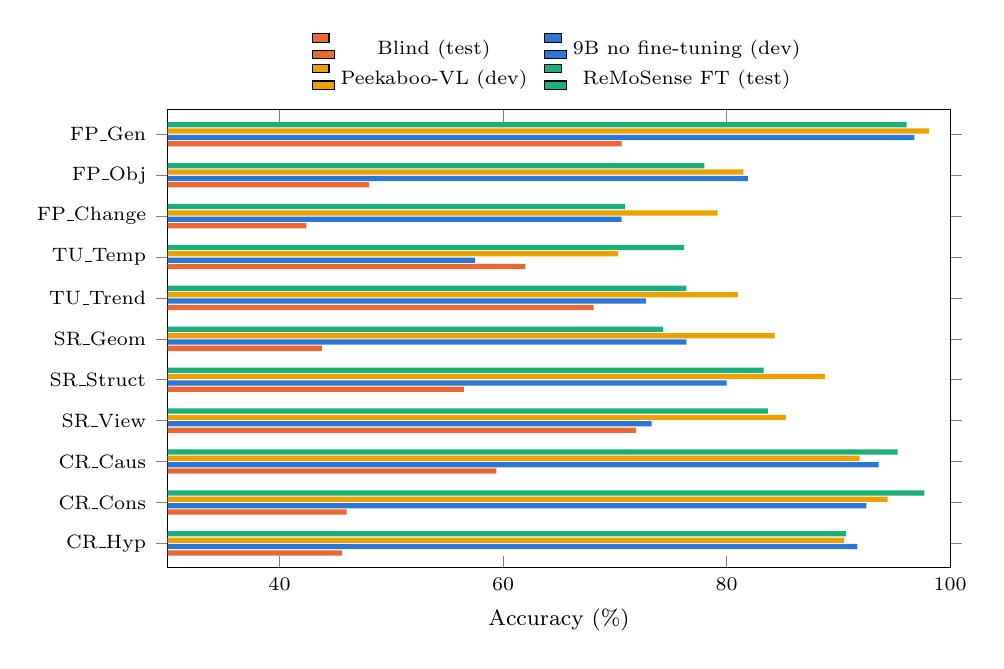
\begin{tikzpicture}
\begin{axis}[
  width=0.95\columnwidth, height=74mm,
  xbar=0.4pt, bar width=1.9pt,
  xmin=30, xmax=100, xtick={40,60,80,100},
  xlabel={Accuracy (\%)}, xlabel style={font=\footnotesize},
  symbolic y coords={CR\_Hyp,CR\_Cons,CR\_Caus,SR\_View,SR\_Struct,SR\_Geom,TU\_Trend,TU\_Temp,FP\_Change,FP\_Obj,FP\_Gen},
  ytick=data, yticklabel style={font=\scriptsize}, xticklabel style={font=\scriptsize},
  legend style={font=\scriptsize, at={(0.5,1.02)}, anchor=south, legend columns=2, draw=none, /tikz/every even column/.append style={column sep=4pt}},
  enlarge y limits=0.06,
]
\addplot[fill=s2, draw=none] coordinates {(45.6,CR\_Hyp) (46.0,CR\_Cons) (59.4,CR\_Caus) (71.9,SR\_View) (56.5,SR\_Struct) (43.8,SR\_Geom) (68.1,TU\_Trend) (62.0,TU\_Temp) (42.4,FP\_Change) (48.0,FP\_Obj) (70.6,FP\_Gen)};
\addplot[fill=s1, draw=none] coordinates {(91.7,CR\_Hyp) (92.5,CR\_Cons) (93.6,CR\_Caus) (73.3,SR\_View) (80.0,SR\_Struct) (76.4,SR\_Geom) (72.8,TU\_Trend) (57.5,TU\_Temp) (70.6,FP\_Change) (81.9,FP\_Obj) (96.8,FP\_Gen)};
\addplot[fill=s4, draw=none] coordinates {(90.5,CR\_Hyp) (94.4,CR\_Cons) (91.9,CR\_Caus) (85.3,SR\_View) (88.8,SR\_Struct) (84.3,SR\_Geom) (81.0,TU\_Trend) (70.3,TU\_Temp) (79.2,FP\_Change) (81.5,FP\_Obj) (98.1,FP\_Gen)};
\addplot[fill=s3, draw=none] coordinates {(90.7,CR\_Hyp) (97.7,CR\_Cons) (95.3,CR\_Caus) (83.7,SR\_View) (83.3,SR\_Struct) (74.3,SR\_Geom) (76.4,TU\_Trend) (76.2,TU\_Temp) (70.9,FP\_Change) (78.0,FP\_Obj) (96.1,FP\_Gen)};
\legend{Blind (test), 9B no fine-tuning (dev), Peekaboo-VL (dev), ReMoSense FT (test)}
\end{axis}
\end{tikzpicture}
\caption{Accuracy per task: our blind scorer on the test leaderboard,
Qwen3.5-9B before and after our fine-tuning (final Peekaboo-VL, PriDe) on dev, and
ReMoSense after fine-tuning on test. Exact values are in
Table~\ref{tab:pertask}.}
\label{fig:pertask}
\end{figure}


\begin{table*}[t]
\centering
\caption{Accuracy per task (\%). Dev for our models (2,078 questions); test for the blind
scorer's leaderboard entry and for ReMoSense~\cite{yao2026reva}. Best per column in bold.}
\label{tab:pertask}
\footnotesize
\setlength{\tabcolsep}{4pt}
\begin{tabular}{@{}lrrrrrrrrrrrr@{}}
\toprule
System & GU & OR & CD & TG & TP & GR & SL & PV & CA & CO & HR & Overall \\
\midrule
Blind text scorer (test) & 70.6 & 48.0 & 42.4 & 62.0 & 68.1 & 43.8 & 56.5 & 71.9 & 59.4 & 46.0 & 45.6 & 55.9 \\
Qwen3.5-4B, no fine-tuning & 94.8 & 80.2 & 67.1 & 51.1 & 73.9 & 68.5 & 80.0 & 71.2 & 90.8 & 91.3 & 90.5 & 77.0 \\
Qwen3.5-9B, no fine-tuning & 96.8 & 81.9 & 70.6 & 57.5 & 72.8 & 76.4 & 80.0 & 73.3 & 93.6 & 92.5 & \textbf{91.7} & 79.6 \\
First model (9B, fine-tuned, 16 frames) & \textbf{99.4} & \textbf{83.9} & \textbf{80.1} & 67.6 & \textbf{82.6} & 80.9 & 88.2 & 83.8 & 94.2 & 92.5 & 88.2 & 84.7 \\
\textbf{Peekaboo-VL} (final, 32 frames, PriDe) & 98.1 & 81.5 & 79.2 & 70.3 & 81.0 & \textbf{84.3} & \textbf{88.8} & \textbf{85.3} & 91.9 & 94.4 & 90.5 & \textbf{85.0} \\
\midrule
ReMoSense-7B, fine-tuned (test) & 96.1 & 78.0 & 70.9 & \textbf{76.2} & 76.4 & 74.3 & 83.3 & 83.7 & \textbf{95.3} & \textbf{97.7} & 90.7 & 80.0 \\
\bottomrule
\multicolumn{13}{@{}p{0.98\textwidth}@{}}{\scriptsize GU General, OR ObjectLand, CD Change, TG Temporal Grounding, TP Trend\,\&\,Pattern, GR Geometric, SL Structural, PV Viewpoint, CA Causation, CO Consequence, HR Hypothetical.}
\end{tabular}
\end{table*}


\subsection{What does fine-tuning add?}
One pass of LoRA training over 8,000 fit questions (500 optimizer steps,
5.2\,h on the A40) lifts Qwen3.5-9B from 79.6\% to \textbf{84.7\%} on dev
(82.3\% test-weighted). The model's predicted letters are spread evenly
over A--D (the KL divergence to a uniform spread is 0.0007, essentially
zero). Because the options were shuffled every time a question was used,
the trained model has no letter preference left to remove: PriDe leaves
accuracy unchanged (84.74\% both ways). On the test set this model
scores 82.6\%. Raw dev accuracy is 2.2 points higher than that, because
dev has relatively more easy questions; the test-weighted dev accuracy
(82.4\% with PriDe) lands within 0.2 points of the test score, which is why
we choose systems by it.

The final model changes three things: 32 frames with a random phase per
training question (Step~1), the drawn clock on Temporal Grounding frames
(Step~4c), and all 14,068 fit questions instead of 8,000. It reaches
85.4\% on dev with plain scores (83.0\% test-weighted) and \textbf{83.6\%}
on the test with PriDe, one point above the first model. Here the
test-weighted dev under-predicted the test by about one point, so we read
dev differences below one point as noise. Temporal Grounding rises from
67.6\% to 70.3\%, Geometric Relation from 80.9\% to 84.3\%, and
Viewpoint from 83.8\% to 85.3\% (Table~\ref{tab:pertask}).

Table~\ref{tab:pertask} shows where the gains come from. They are largest
exactly where the model without fine-tuning was weak: Viewpoint +10.5, Temporal
Grounding +10.1, Trend \& Pattern +9.8, Change Detection +9.5 and
Structural Layout +8.2. Compared with ReMoSense's per-task test numbers,
the dev accuracy of both our models is higher on seven of the eleven tasks. The clear
exception is Temporal Grounding (70.3 for the final model vs.\ 76.2), which we study in
Section~\ref{sec:h6}. The causal tasks are within a few points and hold few
errors.

Why does so little training help so much? Recall that the test asks new
questions about videos that are in the training set. Each training
question teaches the adapter a few facts about one video: where the river
is, what colour the bus is, when the van appears. New questions about the
same video can then reuse these facts. This is allowed by the challenge
rules, and the organizers confirmed that training on these labels is
permitted. What is \emph{not} allowed, and what we do not do, is to look up
training answers about a test clip at test time (``video memory'').

This also tells the reader how to read our margin over ReMoSense. The 9B
backbone without fine-tuning already matches ReMoSense, and fine-tuning on
the seen videos adds about five points. The motion hint's share is small:
removing it from the fine-tuned model costs about 4 of 2,078 dev questions
(Sec.~\ref{sec:cue}). The margin is mostly a newer backbone plus this
training, not evidence that text hints beat learned motion tokens.


\subsection{Why is temporal grounding still hard?}
\label{sec:h6}
To understand the weak Temporal Grounding score, we split the 9B model's answers before fine-tuning
by the type of answer. Questions with an exact time (``at
3.5 seconds'', 102 dev questions) reach 53.9\%. Questions with a time range
(``from 1.0\,s to 4.0\,s'', 57) reach 50.9\%. Questions with a relative
answer (``around the middle'', 60) reach 70.0\%.

When the model picks a wrong exact time, it is usually close: the median
error is 1.0\,s, and 62\% of wrong answers are within 1\,s of the correct
time. That is about the same as the gap between the timestamps the model
sees. With 16 frames there is one timestamp per pair of frames, so every
0.75--1\,s on a typical clip. The model simply cannot tell 3.0\,s from
3.5\,s.
Section~\ref{sec:timetest} tests whether giving the model more time detail
at test time helps.


\subsection{Where are the remaining errors?}
The fine-tuned model makes 317 errors on dev. Temporal Grounding alone has
70 (22\%), followed by Change Detection (45), Object \& Land Cover (39),
Geometric Relation (36), Viewpoint (31) and Trend \& Pattern (30). The
three causal tasks together have 42, and General Understanding only 3.
Fig.~\ref{fig:errors} shows three typical failures.

(a) \emph{A broken clip.} The clip is cut to 0.23\,s (7 frames), but the
correct answer says a van is visible for 4\,s. No model can answer this.
The ten clips shorter than one second carry 137 such questions.

(b) \emph{Counting at dusk.} The vehicles are small and partly hidden, and
it is unclear which ones count as ``parked''. The model counts too few.
This is a known weakness of video models, and a hint with counts from an
object detector is one way to address it.

(c) \emph{Where exactly is it?} The model gets the bus's motion right
(moving away) but puts it at the side of the road instead of the centre
lane. This is a viewpoint error, and a camera-motion hint does not help
with it.

\begin{figure*}[t]
\centering
\footnotesize
\setlength{\tabcolsep}{4pt}
\resizebox{\textwidth}{!}{%
\begin{tabular}{@{}c c c@{}}
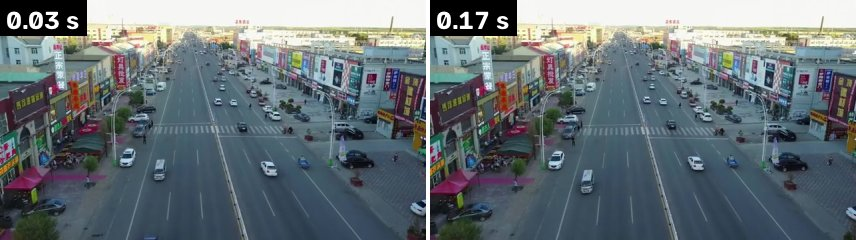
\includegraphics[height=20mm]{figures/failure_truncated.jpg} &
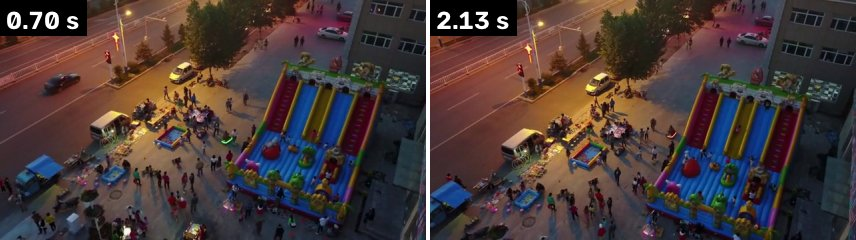
\includegraphics[height=20mm]{figures/failure_count.jpg} &
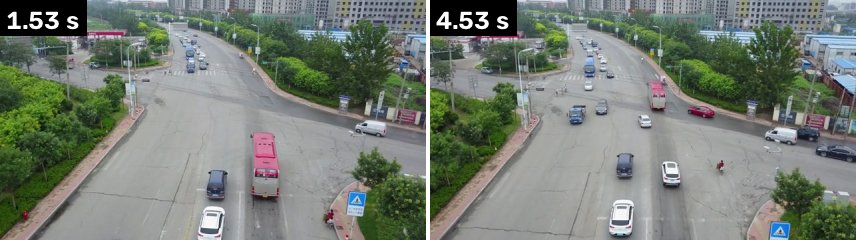
\includegraphics[height=20mm]{figures/failure_bus.jpg} \\[1pt]
\parbox[t]{0.32\textwidth}{\textbf{(a) TU\_Temporal}, 0.23\,s clip. How long is the white van
visible? Correct: \emph{0.0--4.0\,s}. Predicted: \emph{0.0--1.5\,s}.} &
\parbox[t]{0.32\textwidth}{\textbf{(b) FP\_ObjectLand.} How many parked vehicles are visible?
Correct: \emph{5--6}. Predicted: \emph{3--4}.} &
\parbox[t]{0.32\textwidth}{\textbf{(c) FP\_ObjectLand.} Where is the red bus as it moves through
the intersection? Correct: \emph{centre of the frame, toward the top}. Predicted: \emph{right side of
the road, moving away}.} \\
\end{tabular}}
\caption{Three failures of the fine-tuned model on dev: (a) a question that cannot be answered
because the clip is cut short, (b) counting too few small objects at dusk, (c) placing an object
in the wrong spot even though its motion is right. Labels give true times.}
\label{fig:errors}
\end{figure*}


\subsection{How good is the motion measurement on its own?}
Separately from any video model, we checked the motion probe against the
correct answers. We used the 862 training and validation camera-motion
questions whose answer is one of six classes: forward, backward, pan left,
pan right, rotating or stationary. From the probe's summary numbers alone,
we picked a class for each clip (Table~\ref{tab:confusion}).

The probe picks the correct class 73.0\% of the time. Always saying the
most common class (``forward'') would give 57.0\%. When we choose the
option that matches the probe's class, it answers 66.5\% of these questions
correctly (chance is 25\%). Forward flight is recognized in 454 of 491
cases.

Pans are the weak spot. In 60 of 111 ``panning right'' clips, the forward
part of the motion is larger in the clip summary, so the probe says
``forward''. We tried twice to fix this, both times with a pre-registered
plan, and both attempts failed or were inconclusive. Features that describe
the path separate the classes on average (the ratio of sideways to vertical
movement is 0.49 for pans vs.\ 0.14 for forward flight), but the two groups
overlap too much. Looking at the videos showed a deeper problem: on tilted
views, turning the camera (yaw) changes the perspective of the scene. Our
four-number model cannot represent that, so it reports a mix of pan and
rotation.

\begin{table}[t]
\centering
\caption{Motion probe alone vs.\ correct camera-motion answers (862
train+val questions; rows: correct class, columns: probe).}
\label{tab:confusion}
\footnotesize
\setlength{\tabcolsep}{4pt}
\begin{tabular}{@{}lrrrrrr@{}}
\toprule
 & back. & forw. & pan L & pan R & rot. & still \\
\midrule
backward ($n{=}23$) & \textbf{13} & 5 & 1 & 0 & 0 & 4 \\
forward ($n{=}491$) & 4 & \textbf{454} & 6 & 10 & 7 & 10 \\
pan left ($n{=}40$) & 4 & 15 & \textbf{9} & 2 & 4 & 6 \\
pan right ($n{=}111$) & 7 & 60 & 4 & \textbf{25} & 6 & 9 \\
rotating ($n{=}23$) & 1 & 5 & 2 & 1 & \textbf{13} & 1 \\
stationary ($n{=}174$) & 11 & 39 & 1 & 3 & 5 & \textbf{115} \\
\bottomrule
\end{tabular}
\end{table}

% Peekaboo-VL report: 07_ablation. Included from ../peekaboo_report.tex.
\section{Ablation Study}
\label{sec:ablation}
This section changes one part of the system at a time and measures what
it is worth. Not every change could be tested on the full 9B model: the
first hint experiments ran on the small 0.8B model, and the newer training
experiments use the faster packed recipe (Sec.~\ref{sec:packing}) instead
of the 5.2-hour first 9B run, and the last block uses the final recipe. So
each row in Table~\ref{tab:ablation} names its own reference, and only rows
with the same reference should be compared with each other.

\begin{table}[t]
\centering
\caption{All ablations in one place. Each block changes one part of the
system; ``Ref.'' is the reference score (\%) and $\Delta$ the change in
points. FT = fine-tuned, TW = test-weighted dev.}
\label{tab:ablation}
\footnotesize
\setlength{\tabcolsep}{3pt}
\begin{tabular}{@{}p{0.47\columnwidth}p{0.25\columnwidth}rr@{}}
\toprule
Change & Measured on & Ref. & $\Delta$ \\
\midrule
\multicolumn{4}{@{}l}{\textit{Language model} (Sec.~\ref{sec:backbone}); reference Qwen3.5-9B} \\
Cosmos-Reason2-8B & no FT, dev & 79.6 & $-2.7$ \\
Qwen3.8-27B, 4-bit & no FT, dev & 79.6 & $-2.1$ \\
Qwen3.5-4B & no FT, dev & 79.6 & $-2.6$ \\
Cosmos-Reason2-8B & FT packed, TW & 81.6 & $-0.7$ \\
\midrule
\multicolumn{4}{@{}l}{\textit{Camera-motion hint} (Sec.~\ref{sec:cue}); camera-motion questions (88)} \\
Answer words, not image words & 0.8B no FT & 55.7 & $+15.9$ \\
Answer-worded hint vs.\ no hint & 0.8B no FT & 68.2 & $+3.4$ \\
Hint of a wrong clip & 9B FT & 85.2 & $-13.6$ \\
Hint removed & 9B FT & 85.2 & $-4.5$ \\
\midrule
\multicolumn{4}{@{}l}{\textit{Time detail at test time} (Sec.~\ref{sec:timetest}); exact/range TG (159)} \\
32 frames instead of 16 & 9B FT & 67.3 & $-5.0$ \\
Jitter, 3 frame positions & 9B FT & 67.3 & $-4.4$ \\
\midrule
\multicolumn{4}{@{}l}{\textit{Text prior mixed in} (Sec.~\ref{sec:prior})} \\
$\alpha{=}0.75$ fixed in advance & 0.8B no FT, subset & 71.6 & $+6.0$ \\
$\alpha$ by cross-validation & 9B no FT, dev & 79.6 & $+0.6$ \\
$\alpha$ by cross-validation & 9B FT, dev & 84.7 & $+0.4$ \\
\midrule
\multicolumn{4}{@{}l}{\textit{Training recipe} (Sec.~\ref{sec:packing})} \\
8 questions per video (packing) & 9B FT, TW & 82.4 & $-0.8$ \\
Learning rate $2{\times}10^{-4}$ (was $10^{-4}$) & 9B FT packed, TW & 81.6 & $-3.3$ \\
\midrule
\multicolumn{4}{@{}l}{\textit{Object-motion hint} (Sec.~\ref{sec:objmotion})} \\
Object-motion hint added & 9B FT packed, TW & 81.6 & $-0.9$ \\
\midrule
\multicolumn{4}{@{}l}{\textit{On the final recipe} (Sec.~\ref{sec:final-ablation})} \\
Second training pass & final FT, TW & 83.0 & $-0.1$ \\
Caption hint, dev (PriDe) & final FT & 85.0 & $+0.4$ \\
Caption hint, test questions in val & final FT, 392 Q & 80.6 & $-1.8$ \\
64 frames at test (TG, TP, CD) & final FT, 634 Q & 76.7 & $+0.5$ \\
QA-generator model, Qwen3-VL-30B-A3B & no FT, dev & 79.6 & $+0.4$ \\
\bottomrule
\end{tabular}
\end{table}


\subsection{Which language model?}
\label{sec:backbone}
Our method does not depend on one particular model: the hint, the letter
scoring and the LoRA recipe work with any video language model that reads
frames with timestamps. We therefore tried several backbones
(Table~\ref{tab:backbone}).

Without fine-tuning, Qwen3.5-9B is the strongest. The larger Qwen3.8-27B, run
in 4-bit to fit on our GPU, scores lower (77.5\%), and the smaller
Qwen3.5-4B scores 77.0\%. We also tried NVIDIA's
Cosmos-Reason2-8B~\cite{nvidia2025cosmosreason2}, a Qwen3-VL-8B model with
extra training on real-world physical video such as traffic and robots.
Without fine-tuning it scores 76.9\%, 2.7 points below Qwen3.5-9B; it is
weaker on Viewpoint ($-11.5$) and the reasoning tasks, but slightly better
on Trend \& Pattern ($+2.7$).

We then fine-tuned Cosmos-Reason2-8B with exactly the same recipe as a
Qwen3.5-9B run (8 questions per video in one sequence;
Sec.~\ref{sec:packing}). Fine-tuning helps it even more than Qwen (+7.6
test-weighted), but it still ends 0.7 points below Qwen3.5-9B with the same
recipe and 1.5 points below our first unpacked Qwen3.5-9B model. Almost all of the
gap comes from one task, Change Detection ($-8.7$). On Viewpoint, Trend \&
Pattern, Object \& Land Cover and Temporal Grounding it is 1--2 points
\emph{better}, which makes it a promising partner for combining two models.
Qwen3.5-9B remains our main model and is the one behind our test score.

\begin{table}[t]
\centering
\caption{Language models we tried (dev accuracy \%; TW = test-weighted).
``Packed'' runs put 8 questions per video in one training sequence.}
\label{tab:backbone}
\footnotesize
\setlength{\tabcolsep}{4pt}
\begin{tabular}{@{}lrr@{}}
\toprule
Model & Dev & TW \\
\midrule
\multicolumn{3}{@{}l}{\textit{No fine-tuning}} \\
Qwen3.5-4B & 77.0 & -- \\
Qwen3.8-27B (4-bit) & 77.5 & -- \\
Cosmos-Reason2-8B & 76.9 & 73.3 \\
\textbf{Qwen3.5-9B} & 79.6 & -- \\
Qwen3-VL-30B-A3B (FP8; + caption hint) & \textbf{80.0} & 76.8 \\
\midrule
\multicolumn{3}{@{}l}{\textit{Fine-tuned, packed recipe}} \\
Cosmos-Reason2-8B & 83.4 & 80.9 \\
\textbf{Qwen3.5-9B} & \textbf{84.3} & \textbf{81.6} \\
\midrule
\multicolumn{3}{@{}l}{\textit{Fine-tuned, unpacked}} \\
Qwen3.5-9B, first model (16 frames) & 84.7 & 82.4 \\
\textbf{Qwen3.5-9B}, final (32 frames, plain) & \textbf{85.4} & \textbf{83.0} \\
\bottomrule
\end{tabular}
\end{table}


\subsection{Does the wording of the hint matter?}
\label{sec:cue}
We first tested the motion hint with the small Qwen3.5-0.8B model, without
fine-tuning. We used all 191 dev Viewpoint questions, 88 of which ask about
camera motion, and a control set of 100 causal and general questions that
should not depend on motion (Table~\ref{tab:cue}).

The first wording, which described motion in image terms, made things
\emph{worse}. Accuracy on camera-motion questions fell from 68.2\% to
55.7\%. We looked at the 18 questions that this wording turned from right
to wrong. In 12 of them the correct answer was ``moving forward''. But the
hint never said ``forward''. It said ``pans'' in 16 of them and ``zooms
in'' in 14. The model simply matched words from the hint to words in the
options (``Panning from left to right'', ``Zooming in''). The geometry was
right, but the words pointed to the wrong option.

We then wrote the \emph{same} measurements in the answers' own words. This
raised camera-motion accuracy to 71.6\%. Compared with the image wording,
20 questions went from wrong to right and 6 from right to wrong
($p{=}0.009$). Compared with no hint at all, the gain is small and could be
luck (+3.4 points, $p{=}0.69$). The control questions did not change (89 /
88 / 87\%), so the hint does not distract the model on unrelated
questions.

\begin{table}[t]
\centering
\caption{Effect of the hint's wording, Qwen3.5-0.8B without fine-tuning, dev
(\%): no hint, image wording, camera (answer) wording.}
\label{tab:cue}
\footnotesize
\begin{tabular}{@{}lrrr@{}}
\toprule
Question set ($n$) & No hint & Image & Camera \\
\midrule
Camera-motion Viewpoint (88) & 68.2 & 55.7 & \textbf{71.6} \\
Viewpoint-angle (90) & 41.1 & 45.6 & 44.4 \\
All Viewpoint (191) & 56.0 & 52.4 & \textbf{59.2} \\
Control: causal + general (100) & 89.0 & 88.0 & 87.0 \\
\bottomrule
\end{tabular}
\end{table}

\textbf{Does the trained model actually use the hint?} After fine-tuning,
we scored dev again in two altered ways: with the hint removed, and with
the hint of a different, randomly chosen clip (so every clip gets a wrong
hint; Table~\ref{tab:reliance}). The model uses the hint only where it is
relevant. On camera-motion questions, a wrong hint costs 13.6 points (13
questions lost vs.\ 1 gained, $p{=}0.002$), so the model reads what
the hint says. Removing the hint costs 4.5 points ($p{=}0.34$). So after
training, the frames carry most of the information, and the hint adds a
modest amount where it matters. Change Detection, other Viewpoint questions
and all other tasks do not change (within 1 point). Our pre-registered rule
required a 5-point drop when the hint is removed, so we call this result
inconclusive, but with strong evidence that the model reads the hint's
content.

\begin{table}[t]
\centering
\caption{Does the fine-tuned 9B model rely on the hint? (dev, accuracy \%).}
\label{tab:reliance}
\footnotesize
\begin{tabular}{@{}lrrr@{}}
\toprule
Subset ($n$) & Hint & Removed & Wrong clip's \\
\midrule
Camera-motion Viewpoint (88) & \textbf{85.2} & 80.7 & 71.6 \\
Change Detection (231) & 80.5 & 80.5 & 80.5 \\
Other Viewpoint (103) & 82.5 & 83.5 & 83.5 \\
All other tasks (1,656) & 85.4 & 85.5 & -- \\
\bottomrule
\end{tabular}
\end{table}


\subsection{Does more time detail at test time help?}
\label{sec:timetest}
Section~\ref{sec:h6} showed that wrong exact times are near-misses of
about one timestamp gap. So we tried giving the trained model more time
detail at test time, on its
219 dev temporal questions (Table~\ref{tab:h6}). We tried 32 frames instead
of 16. We also tried ``jitter'': averaging the answers from three views
whose frames are taken at 25\%, 50\% and 75\% of each time segment. Both
made exact-time and range questions \emph{worse}: they fell from 67.3\% to
62.3\% (32 frames) and to 62.9\% (jitter, $p{=}0.039$). Only the relative
questions improved, by up to 6.7 points.

Our explanation: the model was trained on 16 centred frames, so it learned
to read time from that exact layout of timestamps. Moving every timestamp
at test time breaks what it learned. The fix must therefore come during
training: train with 32 frames, or with randomly shifted frames, so the
model learns to read any layout. The final model does both (Step~1), and
its Temporal Grounding accuracy rises from 67.6\% to 70.3\%. For that
model, going further to 64 frames at test time no longer hurts, but it
does not help timing questions either (Sec.~\ref{sec:final-ablation}).

\begin{table}[t]
\centering
\caption{More time detail at test time, dev Temporal Grounding
(fine-tuned 9B, trained at 16 frames; accuracy \%).}
\label{tab:h6}
\footnotesize
\begin{tabular}{@{}lrrr@{}}
\toprule
Condition & All & Exact/range & Relative \\
 & (219) & (159) & (60) \\
\midrule
16 frames, centred (as trained) & \textbf{68.0} & \textbf{67.3} & 70.0 \\
32 frames & 66.2 & 62.3 & \textbf{76.7} \\
Jitter, 3 positions & 65.3 & 62.9 & 71.7 \\
\bottomrule
\end{tabular}
\end{table}


\subsection{Does the text prior help a big model?}
\label{sec:prior}
Mixing the blind scorer into the small 0.8B model (no fine-tuning) added 7.7
points on a 220-question dev subset, with $\alpha$ chosen by
cross-validation (64.1$\to$71.8, $p{=}0.0015$). We repeated the test on 250
new questions with $\alpha{=}0.75$ fixed in advance, and the gain held
(71.6$\to$77.6, $p{=}0.008$). On both sets, accuracy is flat for $\alpha$
between 0.5 and 1.5 (Fig.~\ref{fig:alpha}), so the exact value is not
critical.

With the 9B model, the same mix adds only 0.6 points (79.6$\to$80.1,
$p{=}0.33$). The bigger model already knows most of these text patterns.
After fine-tuning the gain is +0.4 (84.7$\to$85.2, $p{=}0.19$), and the
chosen weight falls to $\alpha{=}0.25$ in every fold. Our pre-registered
rule was to use the mix only if it adds at least 1 point with $p{<}0.05$.
It does not, so the submitted system does not use it.

\begin{figure}[t]
\centering
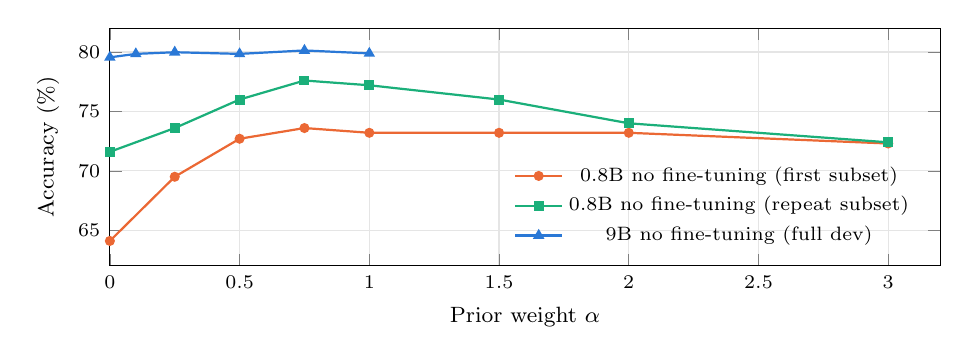
\begin{tikzpicture}
\begin{axis}[
  width=\columnwidth, height=46mm,
  xlabel={Prior weight $\alpha$}, ylabel={Accuracy (\%)},
  xlabel style={font=\footnotesize}, ylabel style={font=\footnotesize},
  ticklabel style={font=\scriptsize},
  xmin=0, xmax=3.2, ymin=62, ymax=82,
  legend style={font=\scriptsize, at={(0.98,0.04)}, anchor=south east, draw=none, fill=none},
  grid=major, grid style={draw=gray!20},
]
\addplot[s2, thick, mark=*, mark size=1.4pt] coordinates {(0,64.1) (0.25,69.5) (0.5,72.7) (0.75,73.6) (1,73.2) (1.5,73.2) (2,73.2) (3,72.3)};
\addplot[s3, thick, mark=square*, mark size=1.4pt] coordinates {(0,71.6) (0.25,73.6) (0.5,76.0) (0.75,77.6) (1,77.2) (1.5,76.0) (2,74.0) (3,72.4)};
\addplot[s1, thick, mark=triangle*, mark size=1.6pt] coordinates {(0,79.55) (0.1,79.84) (0.25,79.98) (0.5,79.84) (0.75,80.13) (1,79.88)};
\legend{0.8B no fine-tuning (first subset), 0.8B no fine-tuning (repeat subset), 9B no fine-tuning (full dev)}
\end{axis}
\end{tikzpicture}
\caption{Accuracy against the weight of the text prior. The gain is large
and stable for the small model and almost disappears at 9B.}
\label{fig:alpha}
\end{figure}


\subsection{Training recipe: packing and learning rate}
\label{sec:packing}
\textbf{One video, many questions per training example.}
Each training example spends about 73\% of its length on video tokens:
roughly 1,920 of 2,000 tokens. Every question about the same clip repeats
the same video tokens. ReVA has about 15 questions per clip, so most of the
compute is spent reading the same frames again and again.

\emph{Question packing} puts the video in once and then asks eight
questions about it, one after another, as a normal chat:
\[
\text{[video] hint } Q_1 \rightarrow A_1,\; Q_2 \rightarrow A_2,\; \ldots,\; Q_8 \rightarrow ?
\]
The model is trained on the answer letter of every question. Because each
question comes after the previous ones, no masking is needed, and the
running memory of the DeltaNet layers is not a problem. We checked that the
first question's scores are the same packed or unpacked (differences within
bf16 rounding). Training becomes 6.4 times faster per question on a small
model. The risk is a mismatch: during training, later questions see other
questions and answers about the same video, which never happens at test
time.

We repeated our main run with packing; the rule written beforehand was
that accuracy must not drop by more than 1 point (test-weighted dev at
least 81.4\%). The packed run reaches 84.3\% on dev and 81.6\% test-weighted, 0.8 points
below the unpacked run (82.4\%) and inside the 1-point margin. Training
took about 70 minutes instead of 5.2\,h, 4.5 times faster. Temporal
Grounding is slightly higher (68.5\% vs.\ 67.6\%). Packing passes, and
because a run now takes about 70 minutes, the packed run is the
reference for the training experiments below. The 0.8-point cost is most
likely a leak: later questions in a pack can see earlier answers about
the same video, which never happens at test time.

\textbf{Learning rate.} Every run so far used a learning rate of
$10^{-4}$, which we never tuned. A recent study that tuned ten LoRA
variants found that, once the learning rate is tuned, plain LoRA is within
one point of all of them~\cite{lee2026lrmatters}; the learning rate
matters more than the variant. We therefore repeated the packed run with
$2{\times}10^{-4}$, changing nothing else. It reached 78.3\% test-weighted,
3.3 points below the packed run at $10^{-4}$ (81.6\%), so we kept
$10^{-4}$. A lower rate ($5{\times}10^{-5}$) was planned but not run.


\subsection{Does an object-motion hint help?}
\label{sec:objmotion}
The ReVA paper names one main failure of video models: confusing the
camera's movement with the movement of objects. Our camera hint tells the
model how the camera moves, but not how the cars move. The
\emph{object-motion hint} does this. For each pair of frames, we
compute dense optical flow (how every pixel moves), fit the ground's
movement with a homography (a transform that also handles tilted views),
and subtract it. Whatever still moves is a moving object. We keep only
small moving blobs that continue in the same direction in the next step,
and describe them by region of the frame and direction, in the questions'
own words:

\smallskip
\noindent\fbox{\parbox{0.95\columnwidth}{\footnotesize\ttfamily
Object motion (camera motion removed): top-right: moving right to left
(0.9-3.9s).}}
\smallskip

\noindent This targets Change Detection and Trend \& Pattern. The hint is
computed for all 1,047 clips: 32 clips have no clearly moving objects and
the median hint is 40 words long. We keep it only if it raises
test-weighted dev by at least 0.5 points (with $p<0.2$), or raises Change
Detection plus Trend \& Pattern by at least 2 points without any task
losing more than 1.5.

\textbf{Result: no gain.} On the plain pass, test-weighted dev falls from
81.6\% to 80.7\% ($-0.9$). With letter debiasing on both runs it is
unchanged (81.0 vs.\ 81.1); each run answers 62 questions the other
misses ($p{=}1.0$). The tasks move in both directions: Structural Layout
$+3.5$ and Geometric Relation $+2.8$, but Object \& Land Cover $-2.8$ and
Change Detection, one of the two target tasks, $-1.3$. Trend \& Pattern
gains only 1.1. Neither rule is met, so the hint is dropped. Two likely
reasons, not yet checked:
after fine-tuning, the frames already show the model how vehicles move,
and on low, tilted views the residual flow still contains parallax from
buildings that the blob filter does not fully remove.



\subsection{What did not help the final model}
\label{sec:final-ablation}
The last block of Table~\ref{tab:ablation} tests four more ideas on the
final recipe. Besides dev, we use a second check that is closer to the
test: the 392 test questions that match a validation question in clip,
question and option set, so their answers are in the official validation
file. The final model answers 316 of them correctly (80.6\%).

\textbf{A second training pass.} Two passes with the learning rate decayed
over both reach 82.96\% test-weighted dev, against 83.04\% for one pass,
and 315 against 316 of the 392 test questions. One pass is enough.

\textbf{A caption hint from the question writer.} ReVA's questions were
written by a large model from video captions. We replayed that captioning
model (Qwen3-VL-30B-A3B) on every clip and gave its caption as a second
hint. Without fine-tuning and without frames, the caption lifts the 9B
model from 64.5\% to 75.9\% on dev (a different clip's caption: 59.3\%),
so the captions carry much of what the questions ask. After fine-tuning,
however, the gain is gone: dev moves by $+0.4$ (85.5\% vs.\ 85.0\%, within
noise), and on the 392 test questions the model with the caption is
\emph{worse} (309 vs.\ 316). We dropped it.

\textbf{More frames at test time.} Scoring the final model with 64 frames
on its three weakest tasks leaves Change Detection unchanged (79.2\%),
moves Temporal Grounding from 70.3\% to 69.9\%, and raises Trend \& Pattern
from 81.0\% to 83.2\%. The last gain rests on 4 questions ($p{=}0.125$), so
we do not count it.

\textbf{The question writer as a second model.} The same 30B model,
without fine-tuning and with both hints, scores 80.0\% on dev, below every
fine-tuned 9B model. Combined with the final model (weights chosen on dev
with folds split by clip), it adds 0.96 test-weighted points on dev
($p{=}0.076$), but only 1 of the 392 test questions. A combination with the
caption-hint model looked better still on dev ($+0.84$, $p{=}0.014$) and
answered one test question \emph{fewer}. On this benchmark, gains of about
one point on dev did not carry over to the test.

% Peekaboo-VL report: 08_discussion. Included from ../peekaboo_report.tex.
\section{Discussion and Limitations}

\textbf{What the video adds.} On ReVA, a text-only model already
reaches 56\% and a 9B video model without fine-tuning 80\%. So most of the remaining
room is in a few tasks: Temporal Grounding, Change Detection and Geometric
Relation. These are exactly the tasks the blind scorer cannot solve. We
suggest that results on ReVA be reported together with a trained blind
baseline and per-task numbers, so readers can see what comes from the
video.

\textbf{Telling instead of learning.} Text hints are cheap, easy to read
and check, and work with any model. But they have two risks that learned
motion tokens do not. First, their wording interacts with the answer
options, as Section~\ref{sec:cue} shows. Second, a wrong hint is stated
just as confidently as a right one. Fine-tuning lets the model learn when
to ignore the hint, and our test with wrong hints shows it does: it follows
the hint on camera-motion questions and ignores it elsewhere.

\textbf{Takeaways we are carrying forward.}
\begin{enumerate}
\item Check how the test relates to the training data before building
anything. Here, the test asks new questions about seen videos, and the
validation set is mostly copies.
\item Build a dev set that copies the test setting, and weight it by the
test's task mix.
\item Train a blind baseline first. It tells you what the video adds and
which tasks need it.
\item When you add text hints, use the words of the answers.
\item Shuffle answer options during training; most letter bias then
disappears, but cheap debiasing (PriDe) still won on the test.
\item Do not trust dev gains of about one point, whether from decoding,
hints or model combinations; several of ours vanished on the test.
\item Do not change the frame layout at test time unless the model was
trained with that layout.
\end{enumerate}

\textbf{Limitations.} Most ablations ran on our first model (57\% of the
fit questions, 16 frames) or on the packed recipe, not on the final model,
so their deltas are directions for the final recipe, not measurements of
it. Our dev split shares clips with the fit set on purpose: it measures
the ``seen video, new question'' setting of this challenge, not how well
the model handles new videos. A fifth of dev are test questions whose
answers the official validation file contains, which makes dev a closer
proxy for the test than a disjoint split would be; we never used those
answers to pick test predictions. We did not use the
training answers about a test clip as context at test time (``video
memory''); the organizers confirmed that this is not allowed, although
training on those labels is. Finally, the probe's four-number motion model
cannot represent camera turns on strongly tilted views; a homography, as
used in our object-motion hint, is the natural next step. Our headline
comparison is against ReMoSense's published numbers rather than a
reproduction, and every configuration is a single seed; both are about our
budget, and both are reasons to read the differences as directions rather
than exact gaps.

\textbf{Broader impact and ethics.} This work studies aerial video
understanding. Drone video is useful for disaster
response, agriculture and traffic monitoring, and it also enables surveillance of
people who did not consent to being recorded. The ReVA dataset is released
for non-commercial research only and may not be redistributed, and we follow
those terms and release no new video data. Our most reusable artifact is a
few-millisecond CPU motion probe that runs on any video. The broader
caution is methodological: when a benchmark's text alone is over half
solvable and its test videos appear in training, reported accuracy can
overstate genuine visual understanding. A recent survey of aerial video
benchmarks~\cite{angelidis2026aerialgap} reached the same conclusion from
the other direction: none of the question-answering benchmarks it audited
reports a blind floor.


% Peekaboo-VL paper: 09_conclusion. Included from ../peekaboo_report.tex.
\section{Conclusion}
We set out to give a video language model the camera motion it cannot see
well, by measuring it and writing it down instead of learning it. A
few-millisecond CPU probe that describes the motion in the answers' own
words, plus LoRA on an off-the-shelf video language model, scores 3.5
points above a purpose-built motion architecture on ReVA, with no new
network parts and one GPU. Most of that margin comes from the newer
backbone and from fine-tuning on the seen videos. The fine-tuned model
does read the hint, but the hint itself adds little.

Three things we learned should hold beyond this benchmark. The test regime
is seen-video, so a development split without training-answer leaks is
essential. Text alone solves 56\%, so the video's real contribution has to
be measured against a blind baseline. And a hint's wording matters more
than the measurement behind it. Temporal grounding remains the weakest
task: training with 32 shifted frames and a drawn clock raised it by 2.7
points, but its errors are still near-misses of about one timestamp. We
hope this encourages more video QA benchmarks to report text-only
baselines and per-task numbers.

The code, the training recipe and the released LoRA adapter are available
at \url{https://github.com/LakoreAI/peekaboo-vl} and
\url{https://huggingface.co/LakoreAI/peekaboo-vl}.


\bibliographystyle{IEEEtran}
\bibliography{refs}

\end{document}
